% Seminar work LaTeX-template for use in seminars in acoustics.
% Thanks go to Jussi Pekonen for editing and updating this template.

% Preferably use a combination of PdfTex and BibTex to compile. This
% can be done easily with a prepared package. Google is your help in
% this case.

% You can modify some things and add packages if you prefer. This setup,
% however, should be enough for most seminar papers. This has been tested
% with current version TeXLive-package (2010), which you should probably 
% use (MacTeX and MikTeX use it). If you do not want to use it, then

%
% Tapani Pihlajamäki 17.1.2011

% Set document class and encoding
\documentclass[11pt,a4paper,twoside]{article}
\usepackage[T1]{fontenc}

% Unicode input encoding
\usepackage{ucs}
\usepackage[utf8x]{inputenc}

% Language. Change to finnish if you write in finnish (or use both)
\usepackage[english]{babel}


% Microtype makes the text really neat.
\usepackage{microtype}

% Graphics package
\usepackage[pdftex]{graphicx}

% Package enabling subfigures. This means that you can use figures
% with automatic "numbering" and referencing.
\usepackage{subfigure}

% Extended equation and symbol functionality
\usepackage{amsmath}
\usepackage{amssymb}



% New fonts based on Aalto
\usepackage{fouriernc}
\usepackage[scaled]{helvet}
\renewcommand*\ttdefault{txtt}
\usepackage{inconsolata}
%\usepackage{tgheros}

% NatBib load. Check NatBib reference with Google if you want to know more
% about its options. In short, it is possible to modify almost everything
% about the citation style.
%\usepackage[round]{natbib}
\usepackage{cite}

% Acoustics style file.
\usepackage{akuseminar}

% Formatting for captions.
\usepackage[hang,bf]{caption}



% Path of graphics files. By default root and figures directory are used.
\graphicspath{{./}{figures/}}

% PDF setup. Generally there should not be any need to change these.
\usepackage[pdftex]{thumbpdf}
\usepackage[pdftex,bookmarks=true,bookmarksnumbered=true,hypertexnames=false,%
  breaklinks=true,linkbordercolor={0 0 0},bookmarksopen=true,%
  hyperfigures=false,colorlinks=true,urlcolor=blue,linkcolor=black,%
  citecolor=black]{hyperref}

% Set stuff for autoref
\addto\extrasenglish{%  
	\def\figureautorefname{Fig.}
	\def\subfigureautorefname{Fig.}
	\def\tableautorefname{Table}
	\def\equationautorefname{Eq.}
	\def\AMSautorefname{Eq.}
	\def\sectionautorefname{section}
	\def\subsectionautorefname{section}
	\def\subsubsectionautorefname{section}
}

% TikZ and pgf plots enable drawing of graphics in TeX. A neat way of producing
% block diagrams and figures, which have the same text formatting as the other
% text. However, this is not mandatory. Comment them in if you want to use them.
%\usepackage{tikz}
%\usepackage{pgfplots}


% Booktabs packages enables a better looking tables, which use less lines and
% more spacing. This is almost standard way of doing tables in text books.
\usepackage{booktabs}








% Paper information. Change these to your own information.

% Change these
\title{Warm Chorus -  Demo}
\author{Aku Rouhe, Niklas Sallinen}
\address{Aalto University School of Electrical Engineering\\
Department of Signal Processing and Acoustics}
\email{niklas.sallinen@aalto.fi}

% These set the properties of the created pdf file.
\hypersetup{%
  pdftitle = {Warm Chorus -  Demo},
  pdfsubject = {Audio Signal Processing Demo Report},
  pdfkeywords = {Music representation, Digital audio workstation, Interactive music},
  pdfauthor = {Aku Rouhe, Niklas Sallinen},
  pdfcreator = {pdf\LaTeX\ using package \flqq hyperref\frqq},
  pdfproducer = {pdf\LaTeX},
}

\pagestyle{plain}

%%%%%%%%%%
% Document
%%%%%%%%%%
\begin{document}

% Create the title based information set above.
\maketitle

% Abstract. Remember that abstract should include the key points of the
% whole article
\begin{abstract}
\noindent\it The Abstract
\end{abstract}

% Keywords, optional. Comment if not needed.
\noindent\textbf{Keywords} --- Keyword 1, keyword 2

% Introduction
\section{Introduction}

Chorus is an effect whose purpose is make sound bigger. It simulates that
instead of one player or singer there are multple ones. 

Richard Dudas was assigned to create chorus effect for New Asia String Quartet to get more
ensemble-like sound for Haydn's Seven Last Words, Op.51, performance. Using a digital effect
was appropriate as they were using amplification and artificial reverb as well. 
As current chorus effects sound unnatural and they have detectable modulation
and beating effects Dudas decided to design new chorus algorithm, Warm Chorus. 
This algorithm is based on physical phenomena rather than just simple mathematical 
consepts. \cite{dudas}

In this report we discuss implementing the Warm Chorus algorithm and how it is
better than current chorus algorithms. As well we describe in detail how we have 
implemented the algorithm.

\clearpage
\section{Theory}
\subsection{Generic Chorus}

Generic chorus algorithm is basd on calcunational motivation. The algorithm has three basic
fuctions. First it multiplies input signal and delays the copies and then detunes those to create
the effect of more than on player. That creates beating effect and other unwanted characteristics into
the sound due to lack of the variance of the parameters used. 

Industry standard chorus is based on delay line modulated with low-frequency oscillator. 
\subsection{Orchestral Section Model}

Orchestral section model is based on real orchestra section and it takes account
placement and playing skills of players. Meaning that the different players play 
different amount out of tune and usually the worst players are placed in the back of
the section.\cite{dudas}

This is completely new way of thinking about chorus as its interest are based on physical
modeling rather than computational tricks. As the current chorus has parameters as modulation 
depth and modulation speed orchestral section model has more real life parameters. Dudas' warm 
chorus algorithm is mainly based on such a model \cite{dudas}.

\clearpage
\section{Implementation}
\begin{figure}[ht]
\centering
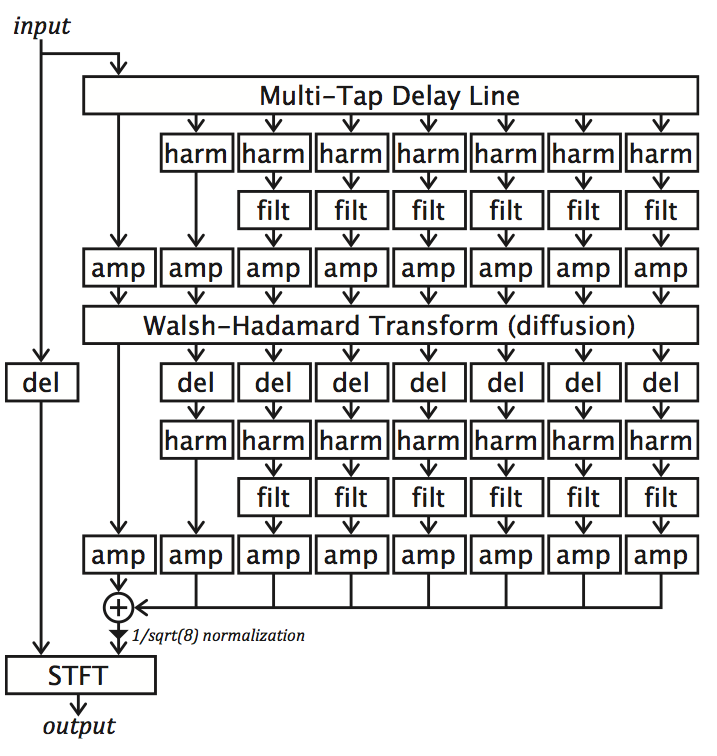
\includegraphics[width= 9cm]{Structure.png}
\caption{Block diagram of the warm chorus algorithm. \cite{dudas}}
\label{fig:struct}
\end{figure}
\subsection{Harmonizer}

Harmonizer is structure which detunes input signal slightly to get different "players" play
slightly out of tune as in the real orchestra section. The block diagram of the harmonizer
is shown in figure \ref{fig_harm}

In harmonizer structure there are four channels which are windowed with four sinusoidal windows
that are 90 degrees more out of phase than previous. To decrease the beating effect that is present
in the current chorus there is added some random variance to the detuning of the sound. That means
that each window is slightly differently out of tune. That is as well related to the real world as the players
usually do not play whole music piece in same detuning. \cite{dudas}
\begin{figure}[ht]
\centering
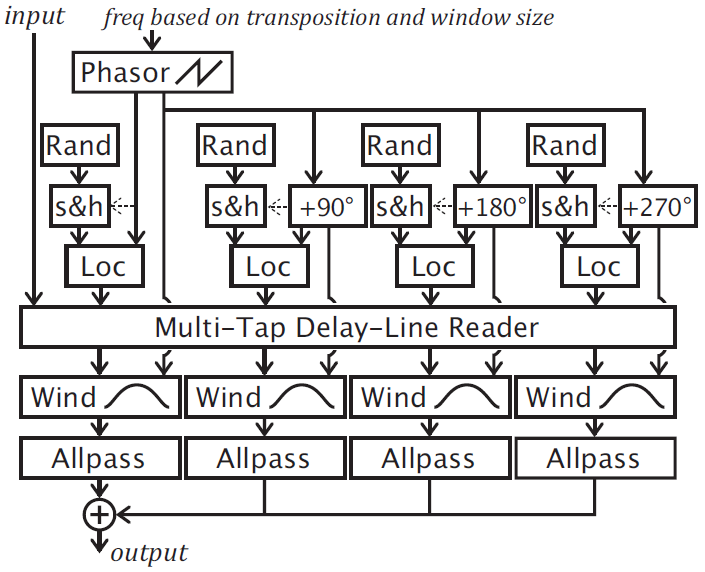
\includegraphics[width = 8cm]{harmonizer.png}
\caption{Chorus Harmonizer Block Diagram. \cite{dudas}}
\label{fig_harm}
\end{figure}

The detuning is made with multi-tap delay-line which is modulated with phasor signal which is basic sawtooth
wave form. After that each channel is windowed by using Hanning window and after that it is allpass filtered.
The windows are triggered with phasor signal and it as well triggers the randomization for each window.
After allpass fitering all the channels are summed together. \cite{dudas}

\subsection{Temporal processing}
In addition to the harmoniser stages, the temporal processing includes a multi-tap delay, low-pass filters, random amplitude ramping and a diffusion stage. These can be seen in fig~\ref{fig:struct}. 


The multi-tap delay line simulates the delays between the players caused by the finite speed of sound \cite{dudas}. We are assuming 340$\frac{m}{s}$. We calculate the delay for the distances of the players, with the distances varying from just over a metre to several metres. The more delayed channels correspond to players at the back of the section. There are infact two delay stages with equal delays. The first simulates the delay for the hearing the section leader, and the second simulates the delay for the sound traveling from the back of the section to the front.


The low-pass filters simulate absorption in the air in a slightly exaggerated manner \cite{dudas}. They are implemented as simple first-order finite impulse response filters. The more delayed paths are filtered more, since they correspond to sounds which travel over a larger distance.

The random amplitude ramping simulates the dynamic variation which human players do naturally. The randomness helps remove audible periodicity \cite{dudas}. The amplitude ramping is done with simple gains which go back-and-forth linearly between two values during randomised time intervals. The more delayed paths, which correspond to worse players, have a higher difference between the maximum and minimum gains, but lower overall volume.

The diffusion stage is used to get a fuller sound. It is based on a hadamard matrix, which is often used in feedback delay networks for the same purpose. \cite{Jot} Here, however, there is no feedback.

Dudas does not relate the diffusion stage to orchestral section modeling. However, we propose the following: since the players hear eachother's pitches all at the same time, they cannot distinguish the one perfectly in-tune reference. The first stage of harmonisers which is then diffused provides the reference pitch, which is already a little ambiguous. Then the second stage of harmonisers is the players' attempt to follow this reference. 

\subsection{Frequency domain processing}
Blah blah


\clearpage
\section{Results}
The algorithm was tested with different audio samples. The most important tests were done with anechoic samples of a single violin player, as this was closest to the original purpose. We also tested the algorithm with samples of recorded electric guitar, and an already heavily processed piece of music. Different parameter values for the algorithm were also tested.

Figure~\ref{fig:dryspec} shows the spectrogram of an uneffected, anechoic violin recording. The partials are clear and the vibrato of the player is also easy to see, particularly around the $2.5s$ time point
\begin{figure}[ht]
\centering
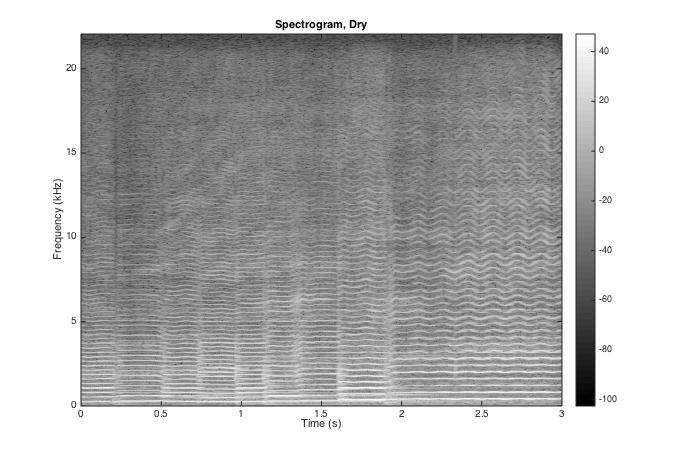
\includegraphics[width=\textwidth]{dry_spec.png}
\caption{Spectrogram of dry signal.}
\label{fig:dryspec}
\end{figure}

Figure~\ref{fig:effspec} shows the spectrogram of the same sample as figure~\ref{fig:dryspec}, but this time passed through the Warm Chorus algorithm. Though the partials are still some what visible, the spectrogram is now more blurry and the vibrato of the original recordings appears to be masked by the effect.
\begin{figure}[ht]
\centering
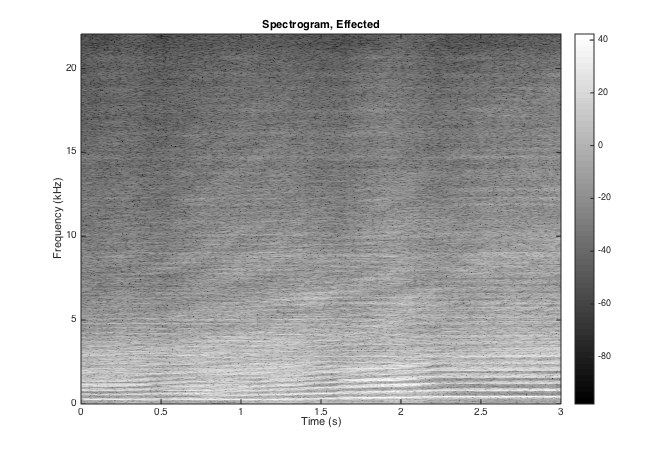
\includegraphics[width=\textwidth]{effected_spec.png}
\caption{Spectrogram of effected signal.}
\label{fig:effspec}
\end{figure}

The blurryness is explained by two factors. Firstly, as is also audible, the algorithm gives the input a reverberated quality due to the reasonably long delays. This blurs the spectrogram in the horisontal direction Secondly, the harmonisers spread the frequency content, which blurs the spectrogram in the vertical direction.

The algorithm's output has no obvious periodic pulse. The output gives the impression of many players playing the same thing in a space. The spaciousness seems inseparable from the impression of a section of players.

When compared with a generic chorus algorithm, the Warm Chorus is much more convincing and realistic. However, the generic chorus has a distinct sound of its own.

When using some extreme settings, the Warm Chorus algorithm may produce quite unpleasant results. After some point, the detuning of the input makes the output sound audibly out-of-tune. Similarly, too much simulated distance between the players results in losing temporal accuracy.




\clearpage
\section{Conclusions}
We implemented the Warm Chorus algorithm as described by Richard Dudas \cite{dudas}. The Matlab implementation fulfilled its primary goal of sounding better and more importantly more realistic than a generic chorus algorithm. The authors feel that the impression of multiple players, which the algorithm strives to provide, is quite convincing in some cases.

The most interesting part in the algorithm's design is the orchestral section modeling, which motivates most choices in the structure. Dudas hopes to inspire other real-world motivated algorithms \cite{dudas} and we join in this thought.

Dudas goes to great lengths in trying to avoid any periodicity in the output; the harmonisers have random characteristics, the frequency domain processing attempts to remove low-end amplitude modulation, the ratios of the parameters are not simple. This works well in the end: the output has no pulse or beating, which aids in not sounding mechanic.

The primary goal for any musical application of digital signal processing is a pleasing sound. This is goal is shown for example in Dudas' use of frequency domain processing techniques for simply removing phasiness. This step might have been excluded were the aim simply to dogmatically imitate an orchestral section. The goal of a good sounding algorithm is a subjective one. The reader is encouraged to listen to sound samples and try the algorithm for herself.




\clearpage
% References. This is done using BibTeX and NatBib package.
% This can be used at the beginning of the seminar to present all references easily.
% Comment out when ready.
%\nocite{*} 
%\renewcommand{\refname}{\vspace{-1cm}\normalsize\section{References}}
% Select style for bibliography. Current is following Harvard-style which is usually used
% in acoustics seminars.
\bibliographystyle{plain}
% Reference to bibliography file.
\bibliography{refs}

%\clearpage
%\begin{thebibliography}{99}
%\bibitem{dudas} Warm Chorus...
%\end{thebibliography}

\end{document}
